\section*{Phase I SARS-CoV-2 HRSM Pilot Summary}

\textbf{Generated:} 2026-06-04

\subsection*{Scope}
This report summarizes the Phase I figure-source reconstruction of the Kemp et al. chronic SARS-CoV-2 infection trajectory. The analysis uses the Fig. 5a workbook sheet from the Kemp figure-source data and should not be described as raw FASTQ or full variant-calling analysis.

\subsection*{Data status}
\begin{itemize}
\item Retained biological rows: 20
\item Removed footer or blank rows: 3
\item Source level: figure-source reconstruction
\item Main mutation pair: D796H and \(\Delta H69/\Delta V70\)
\item CT values: interpolated by explicit day anchors for pilot rebound proxy construction
\item Memory kernel: chronological exponential decay, \(\tau=7\) days, max lag \(=30\) days
\end{itemize}

\subsection*{Main result}
The daily-corrected HRSM trajectory separates the chronic infection into a low-escape baseline, a coherent escape surge at day 82, an alternate diversity state between days 89 and 95, and a retained escape/high-memory return cycle from day 98 onward.

The strongest HRSM contrast is between the alternate diversity state and the retained escape/high-memory return states. The alternate diversity state has high reserve-like diversity but weak or negative memory/coherence, while the retained escape and high-memory return states recover positive memory and coherence around the D796H plus \(\Delta H69/\Delta V70\) structure.

\subsection*{Transition-state summary}
\begin{tabular}{llllllllll}
\toprule
transition\_state & n & first\_day & last\_day & mean\_escape & mean\_H & mean\_R & mean\_S & mean\_M & mean\_Phi \\
\midrule
low\_escape\_baseline & 6 & 1 & 66 & 0.003517 & -1.433 & 0.1647 & -0.7733 & -0.896 & -0.7345 \\
intermediate\_transition & 2 & 55 & 86 & 0.0141 & 0.1003 & 0.3535 & -0.9086 & -0.5975 & -0.2631 \\
coherent\_escape\_surge & 1 & 82 & 82 & 0.9126 & 0.5647 & 0.4617 & 1.548 & 1.595 & 1.042 \\
alternate\_diversity\_state & 4 & 89 & 95 & 0.04381 & 0.786 & 1.264 & -0.2695 & -0.6098 & 0.2926 \\
retained\_escape\_state & 5 & 98 & 101 & 0.6766 & 0.6804 & -0.7474 & 0.6988 & 0.9033 & 0.3838 \\
high\_memory\_escape\_return & 2 & 99 & 101 & 0.8364 & 0.6446 & -1.737 & 1.247 & 1.449 & 0.4009 \\
\bottomrule
\end{tabular}

\subsection*{Daily-collapsed transition matrix}
\begin{tabular}{lllllll}
\toprule
from\_state & low\_escape\_baseline & intermediate\_transition & alternate\_diversity\_state & coherent\_escape\_surge & retained\_escape\_state & high\_memory\_escape\_return \\
\midrule
low\_escape\_baseline & 0.6667 & 0.1667 & 0 & 0.1667 & 0 & 0 \\
intermediate\_transition & 0.5 & 0 & 0.5 & 0 & 0 & 0 \\
alternate\_diversity\_state & 0 & 0 & 0.6667 & 0 & 0.3333 & 0 \\
coherent\_escape\_surge & 0 & 1 & 0 & 0 & 0 & 0 \\
retained\_escape\_state & 0 & 0 & 0 & 0 & 0 & 1 \\
high\_memory\_escape\_return & 0 & 0 & 0 & 0 & 1 & 0 \\
\bottomrule
\end{tabular}

\subsection*{Stationary distribution}
\begin{tabular}{ll}
\toprule
state & stationary\_probability \\
\midrule
retained\_escape\_state & 0.5 \\
high\_memory\_escape\_return & 0.5 \\
intermediate\_transition & 0 \\
low\_escape\_baseline & 0 \\
coherent\_escape\_surge & 0 \\
alternate\_diversity\_state & 0 \\
\bottomrule
\end{tabular}

The stationary distribution is computed by solving the linear stationary equations, not by power iteration. This matters because the daily-collapsed matrix contains a deterministic two-state terminal cycle. The stationary mass is therefore split evenly between retained escape and high-memory escape return.

\subsection*{Velocity summary}
\begin{tabular}{lllllllllllllll}
\toprule
transition\_state & n & first\_day & last\_day & mean\_step\_velocity & median\_step\_velocity & max\_step\_velocity & mean\_calendar\_velocity & median\_calendar\_velocity & max\_calendar\_velocity & mean\_step\_acceleration & max\_step\_acceleration & mean\_calendar\_acceleration & max\_calendar\_acceleration & same\_day\_steps \\
\midrule
low\_escape\_baseline & 6 & 1 & 66 & 1.225 & 1.288 & 2.641 & 0.2488 & 0.1769 & 0.6603 & 0.2231 & 2.391 & 0.01032 & 0.1633 & 0 \\
intermediate\_transition & 2 & 55 & 86 & 2.387 & 2.387 & 3.314 & 0.5603 & 0.5603 & 0.8286 & -0.3213 & 0.3624 & 0.07707 & 0.1397 & 0 \\
coherent\_escape\_surge & 1 & 82 & 82 & 4.319 & 4.319 & 4.319 & 0.2699 & 0.2699 & 0.2699 & 2.841 & 2.841 & 0.008475 & 0.008475 & 0 \\
alternate\_diversity\_state & 4 & 89 & 95 & 1.063 & 1.202 & 1.688 & 0.3891 & 0.3563 & 0.8438 & -0.4067 & 1.526 & 0.08315 & 0.4219 & 1 \\
retained\_escape\_state & 5 & 98 & 101 & 1.534 & 0.5859 & 3.67 & 0.4631 & 0.5187 & 1.223 & 0.1702 & 1.982 & 0.4061 & 0.5732 & 2 \\
high\_memory\_escape\_return & 2 & 99 & 101 & 1.561 & 1.561 & 1.704 & 0.8522 & 0.8522 & 1.704 & -0.5603 & 0.8451 & 0.4811 & 0.4811 & 1 \\
\bottomrule
\end{tabular}

\subsection*{Potential-well summary}
\begin{tabular}{llllllllllllllll}
\toprule
transition\_state & n & first\_day & last\_day & mean\_U & min\_U & max\_U & mean\_Phi & mean\_escape & mean\_step\_velocity & median\_step\_velocity & max\_step\_velocity & mean\_calendar\_velocity & median\_calendar\_velocity & max\_calendar\_velocity & same\_day\_steps \\
\midrule
low\_escape\_baseline & 6 & 1 & 66 & 0.7345 & 0.3931 & 0.8921 & -0.7345 & 0.003517 & 1.225 & 1.288 & 2.641 & 0.2488 & 0.1769 & 0.6603 & 0 \\
intermediate\_transition & 2 & 55 & 86 & 0.2631 & 0.08067 & 0.4455 & -0.2631 & 0.0141 & 2.387 & 2.387 & 3.314 & 0.5603 & 0.5603 & 0.8286 & 0 \\
coherent\_escape\_surge & 1 & 82 & 82 & -1.042 & -1.042 & -1.042 & 1.042 & 0.9126 & 4.319 & 4.319 & 4.319 & 0.2699 & 0.2699 & 0.2699 & 0 \\
alternate\_diversity\_state & 4 & 89 & 95 & -0.2926 & -0.6653 & -0.05897 & 0.2926 & 0.04381 & 1.063 & 1.202 & 1.688 & 0.3891 & 0.3563 & 0.8438 & 1 \\
retained\_escape\_state & 5 & 98 & 101 & -0.3838 & -0.556 & -0.216 & 0.3838 & 0.6766 & 1.534 & 0.5859 & 3.67 & 0.4631 & 0.5187 & 1.223 & 2 \\
high\_memory\_escape\_return & 2 & 99 & 101 & -0.4009 & -0.7965 & -0.00535 & 0.4009 & 0.8364 & 1.561 & 1.561 & 1.704 & 0.8522 & 0.8522 & 1.704 & 1 \\
\bottomrule
\end{tabular}

\subsection*{Figures}
\begin{figure}[h]
\centering
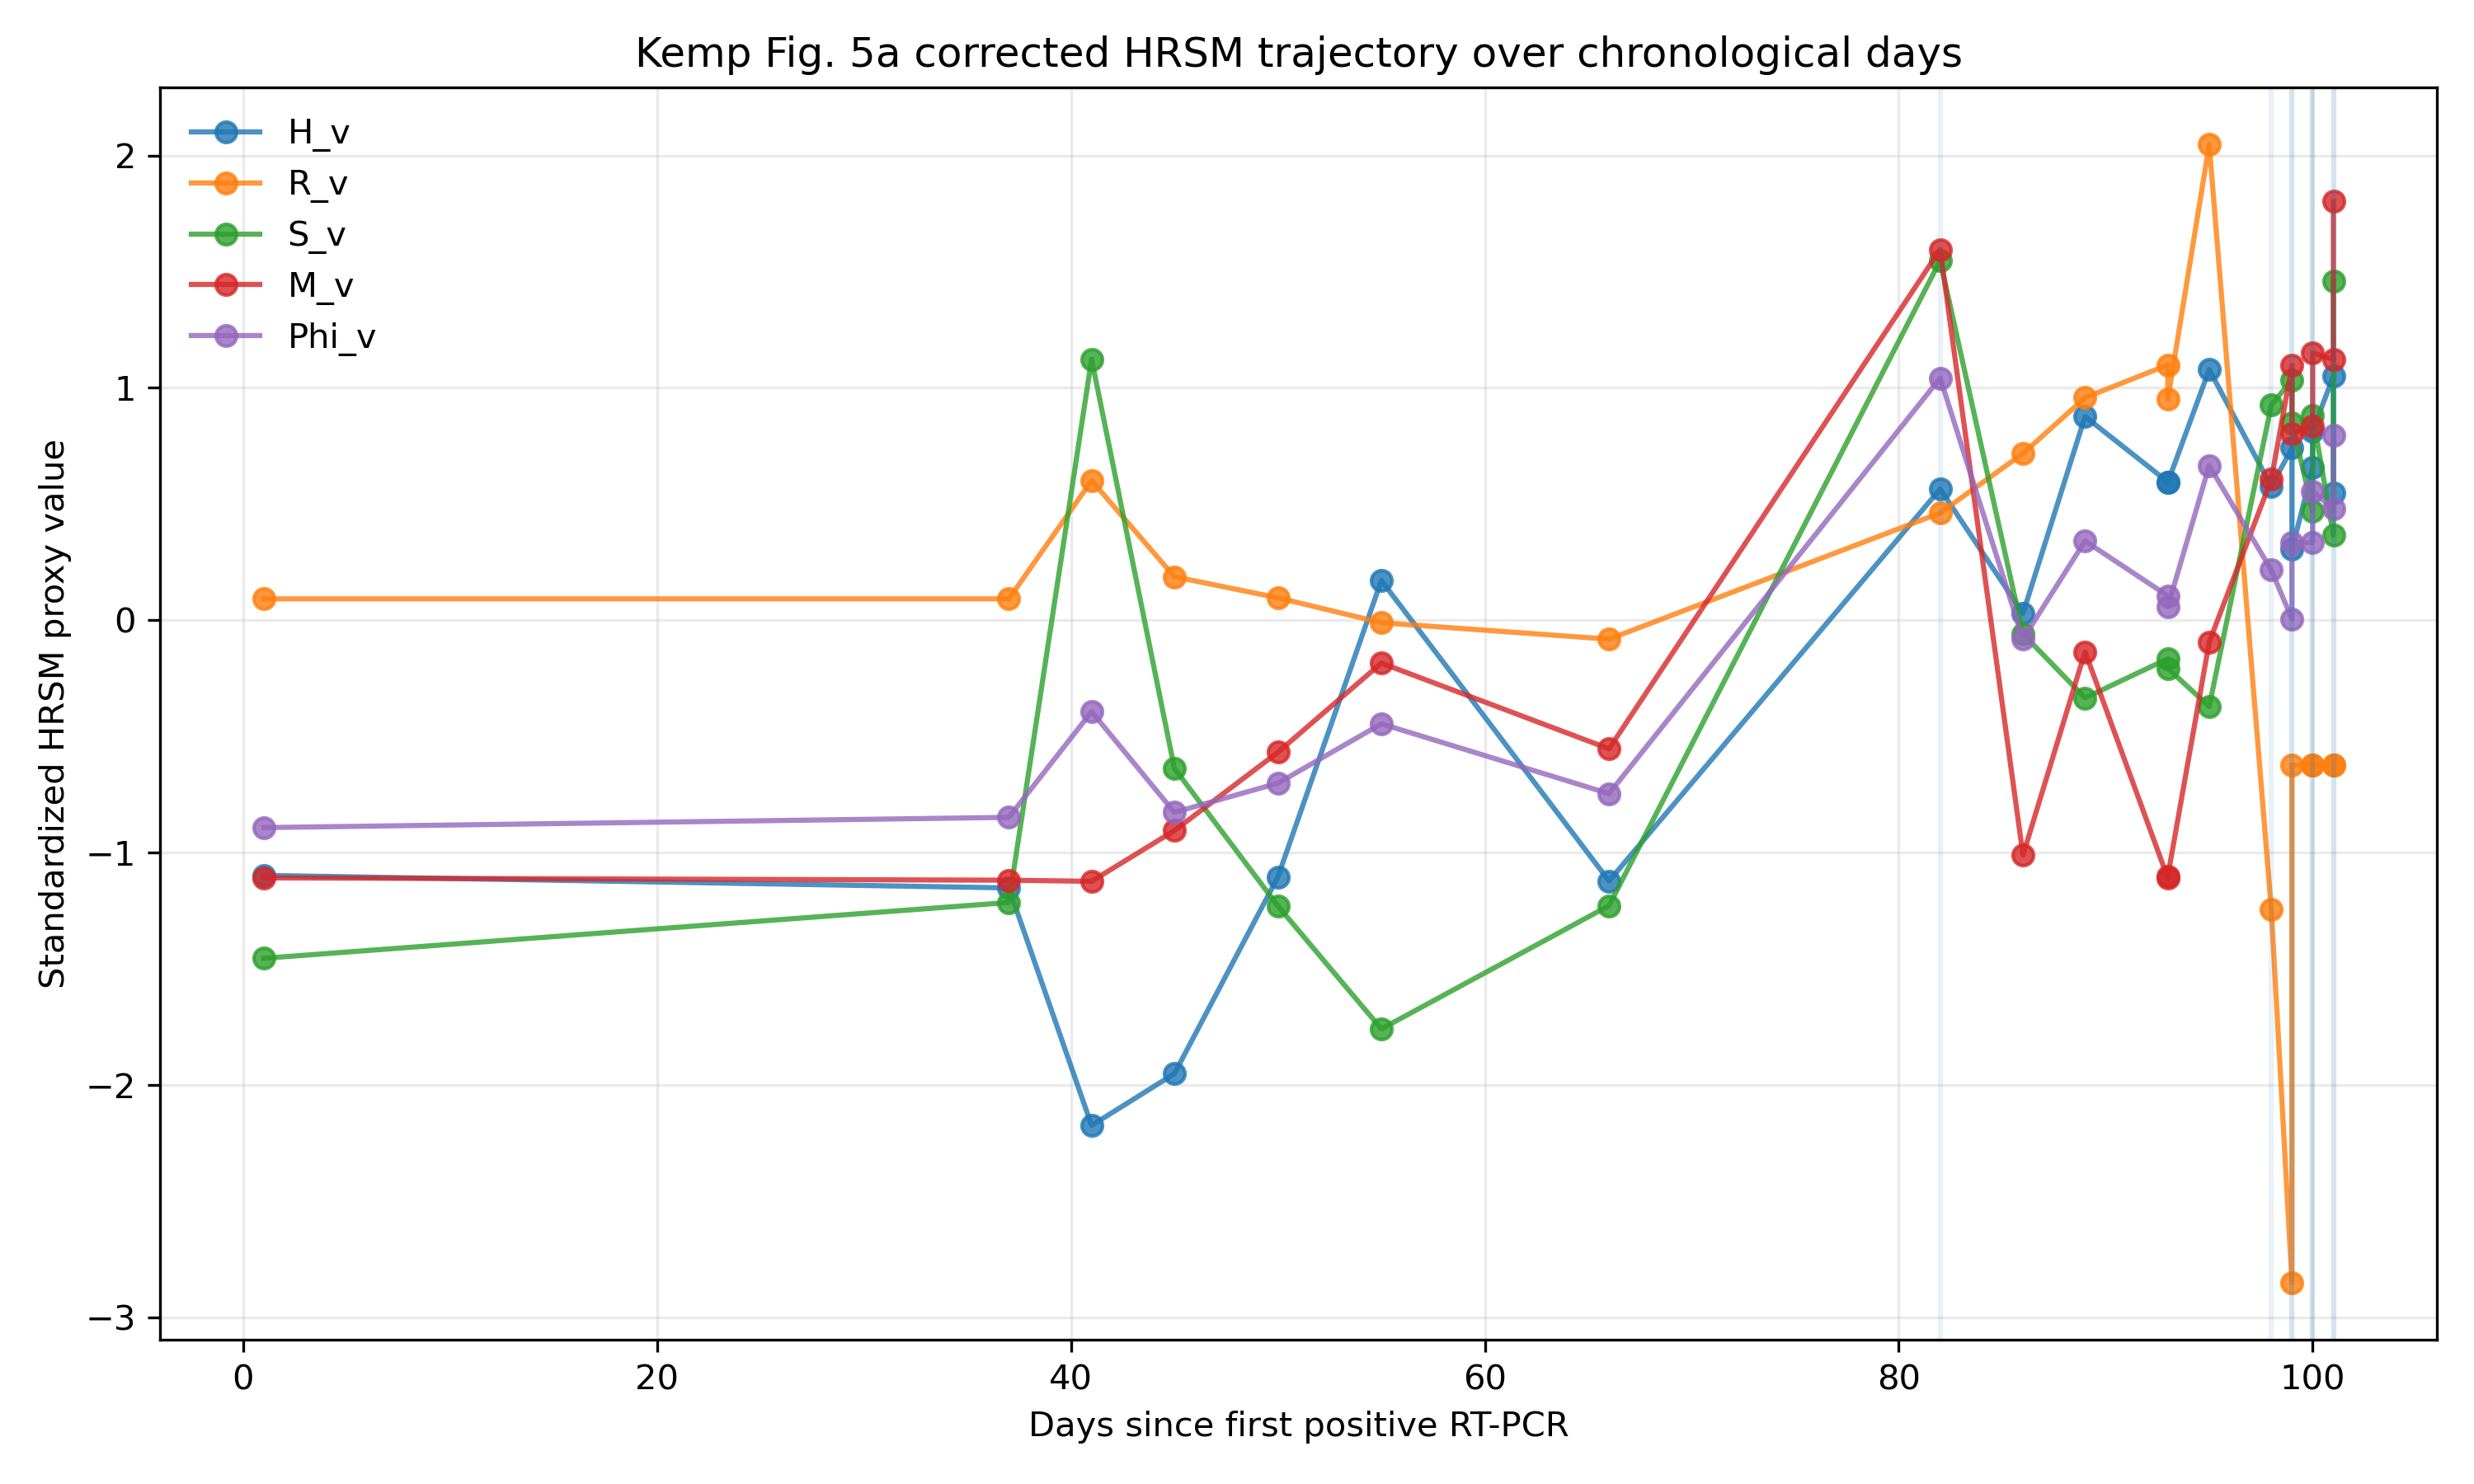
\includegraphics[width=0.9\textwidth]{figures/phase1_sarscov2/kemp_fig5a_colored_hrsm_axes_over_days.png}
\caption{kemp fig5a colored hrsm axes over days}
\end{figure}

\begin{figure}[h]
\centering
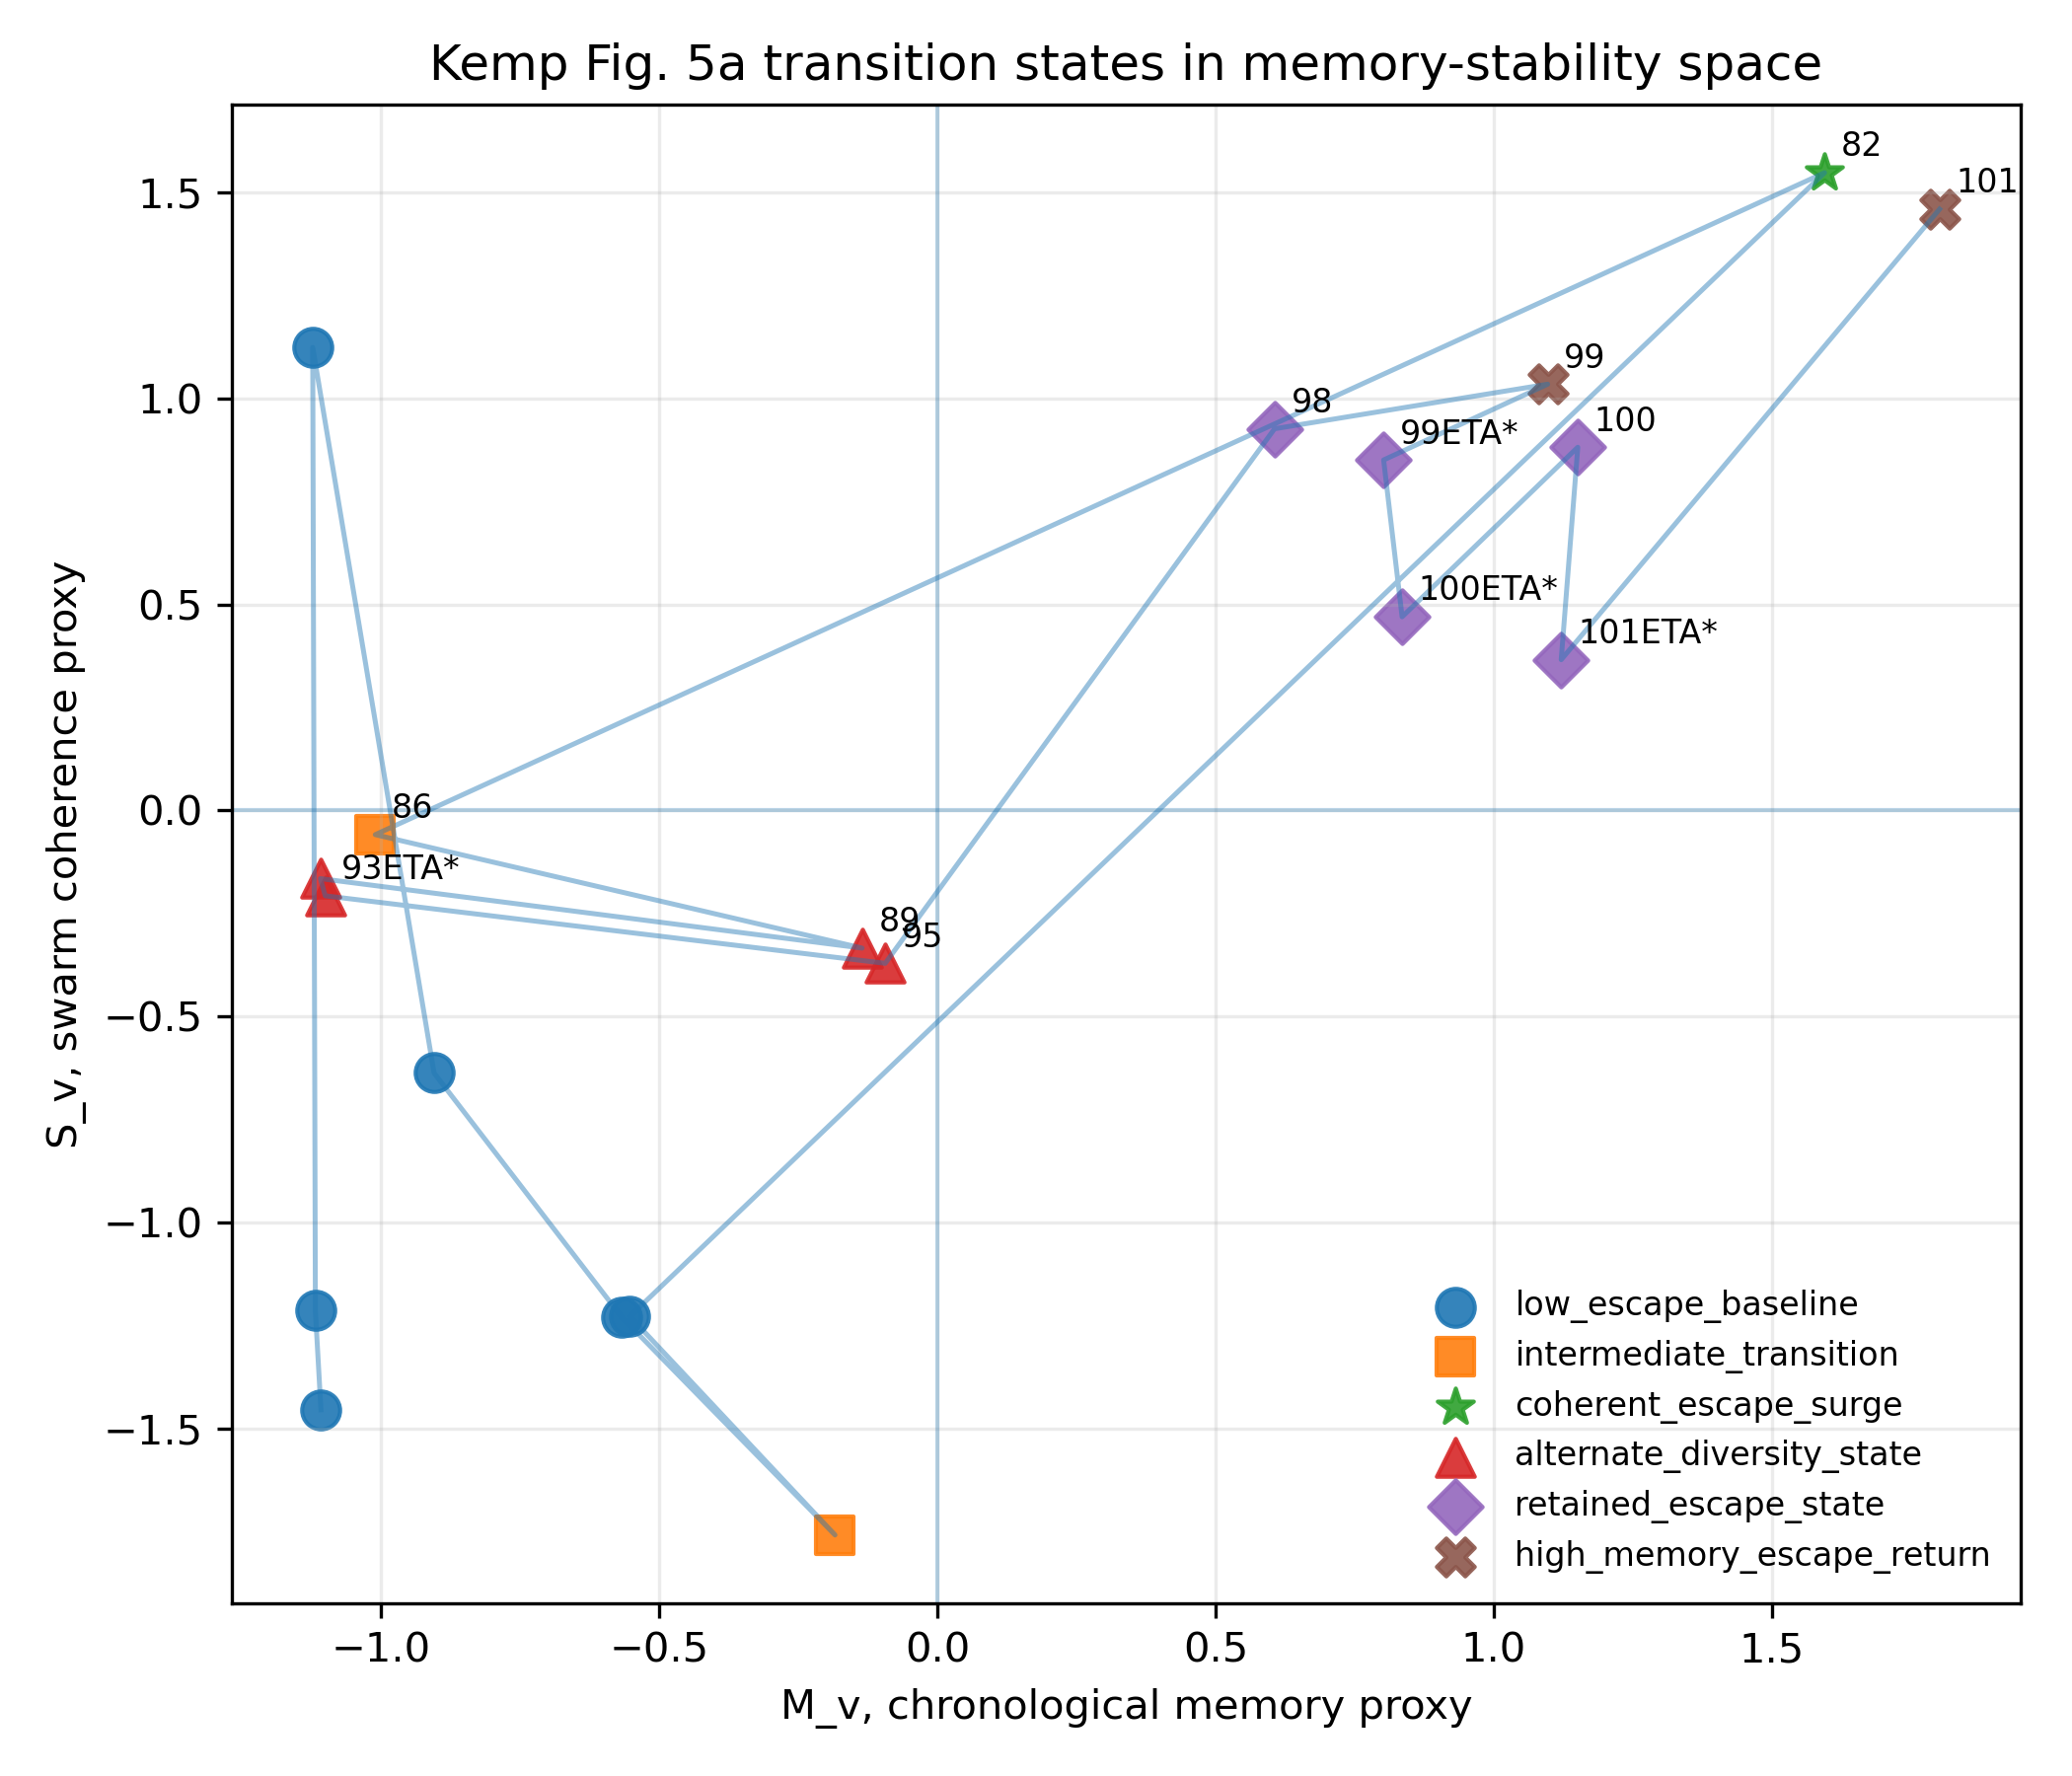
\includegraphics[width=0.9\textwidth]{figures/phase1_sarscov2/kemp_fig5a_colored_memory_stability_states.png}
\caption{kemp fig5a colored memory stability states}
\end{figure}

\begin{figure}[h]
\centering
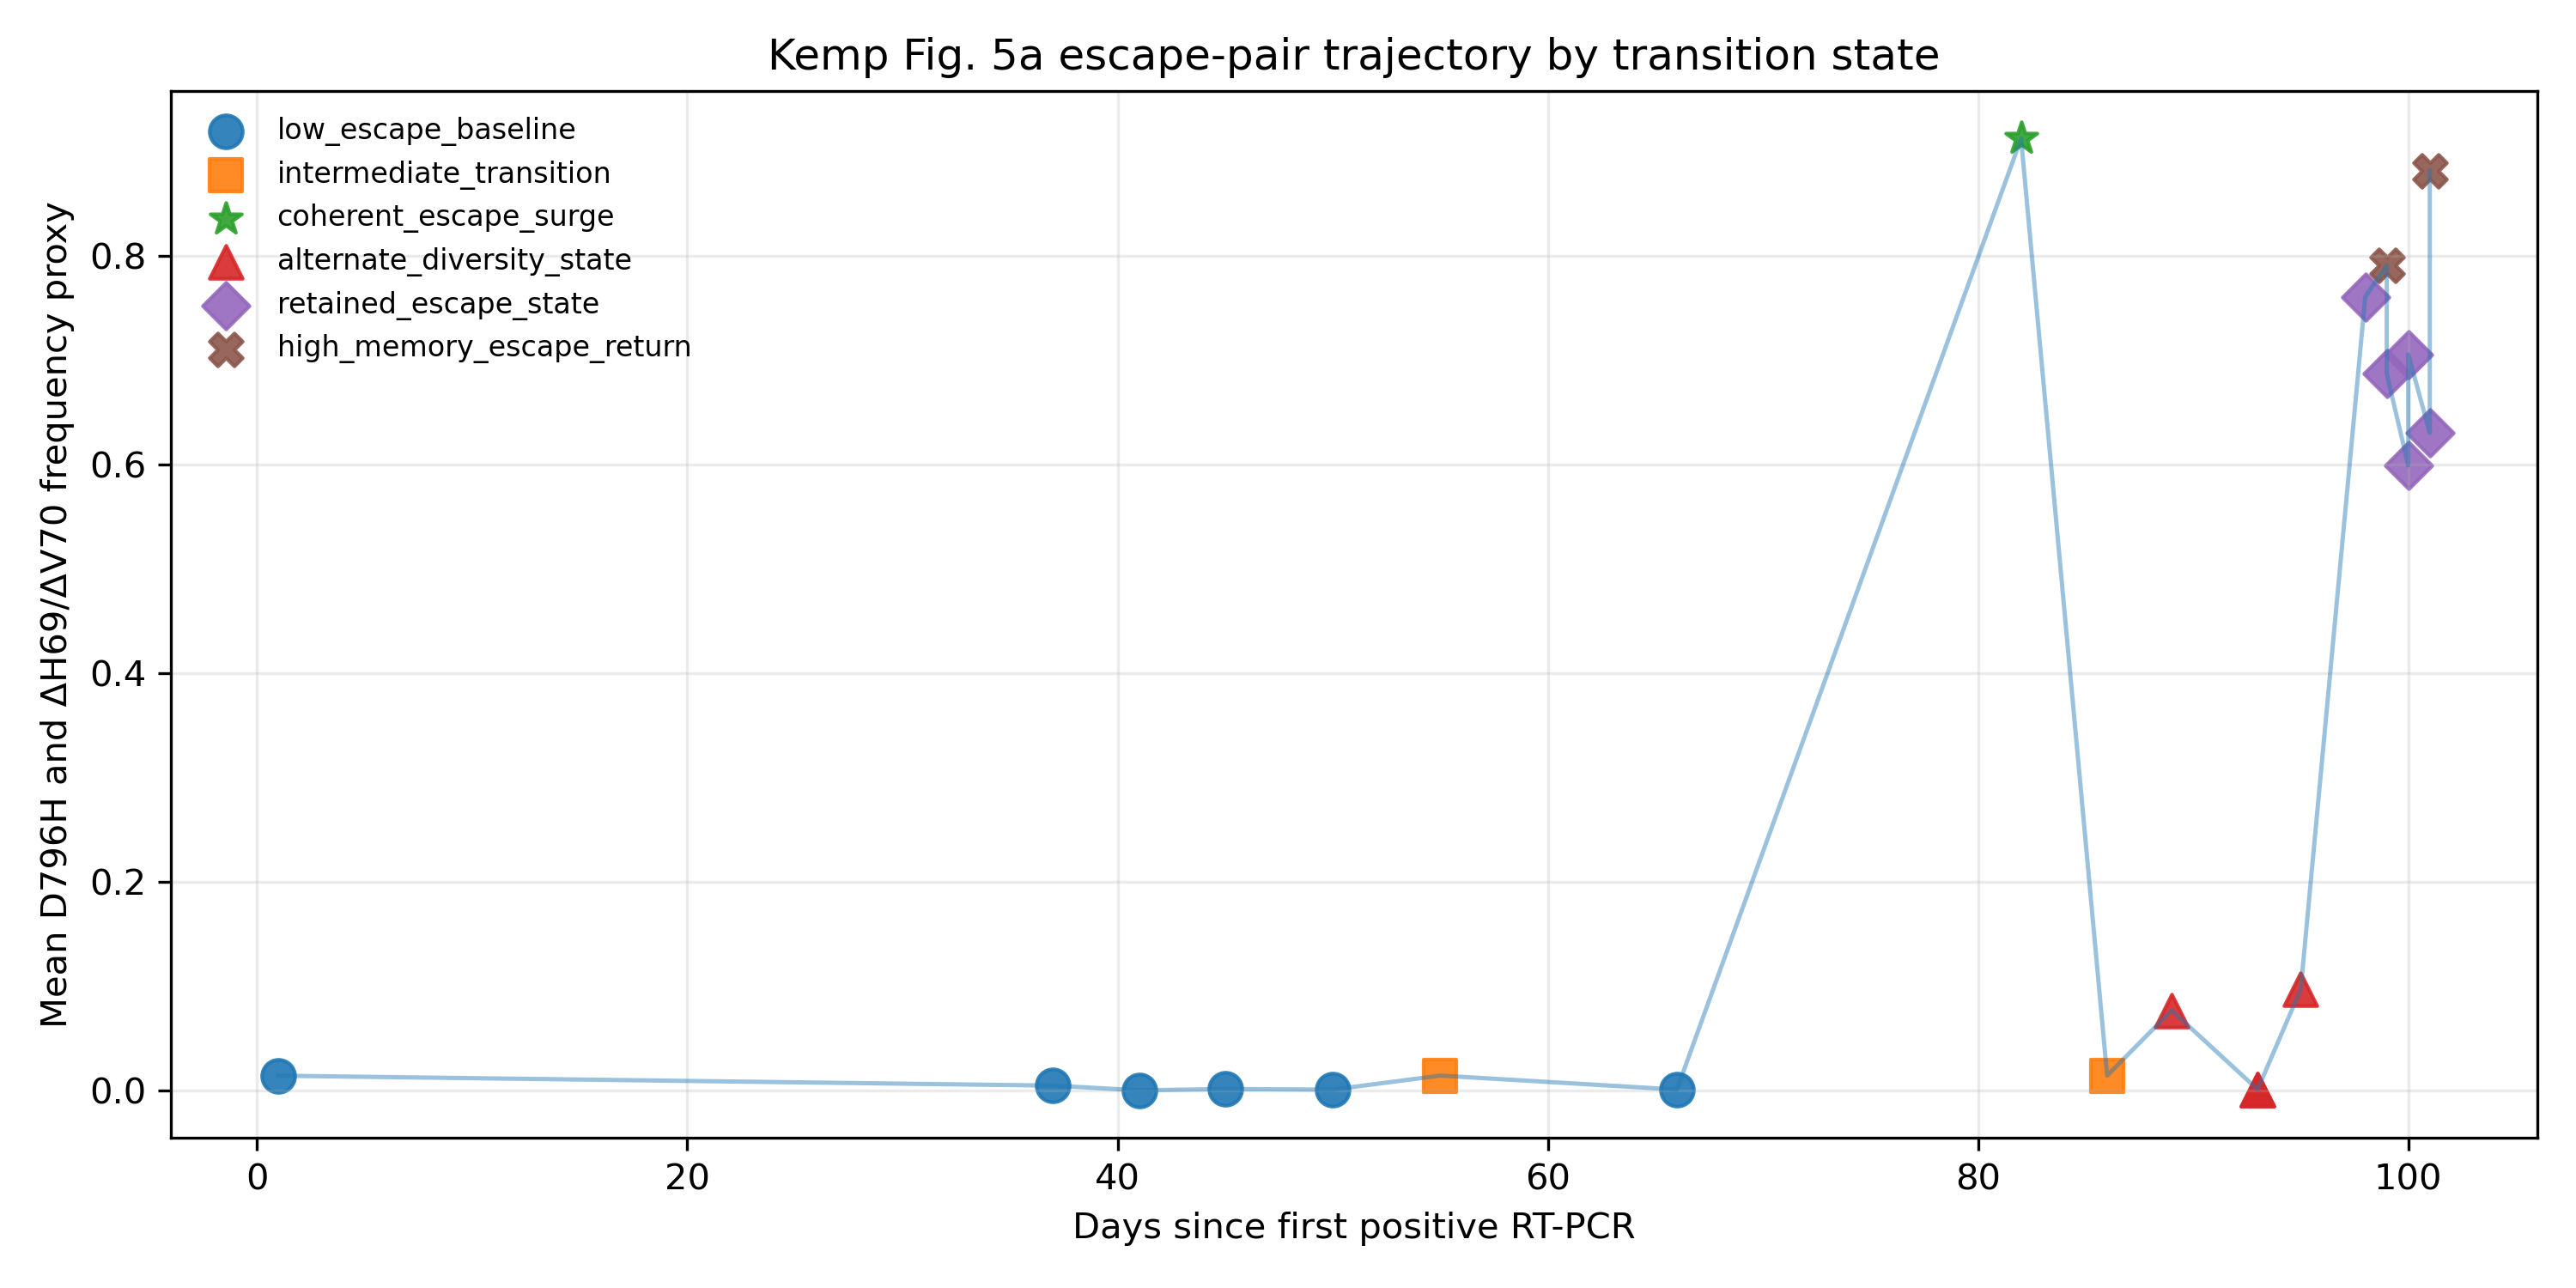
\includegraphics[width=0.9\textwidth]{figures/phase1_sarscov2/kemp_fig5a_colored_escape_memory_over_days.png}
\caption{kemp fig5a colored escape memory over days}
\end{figure}

\begin{figure}[h]
\centering
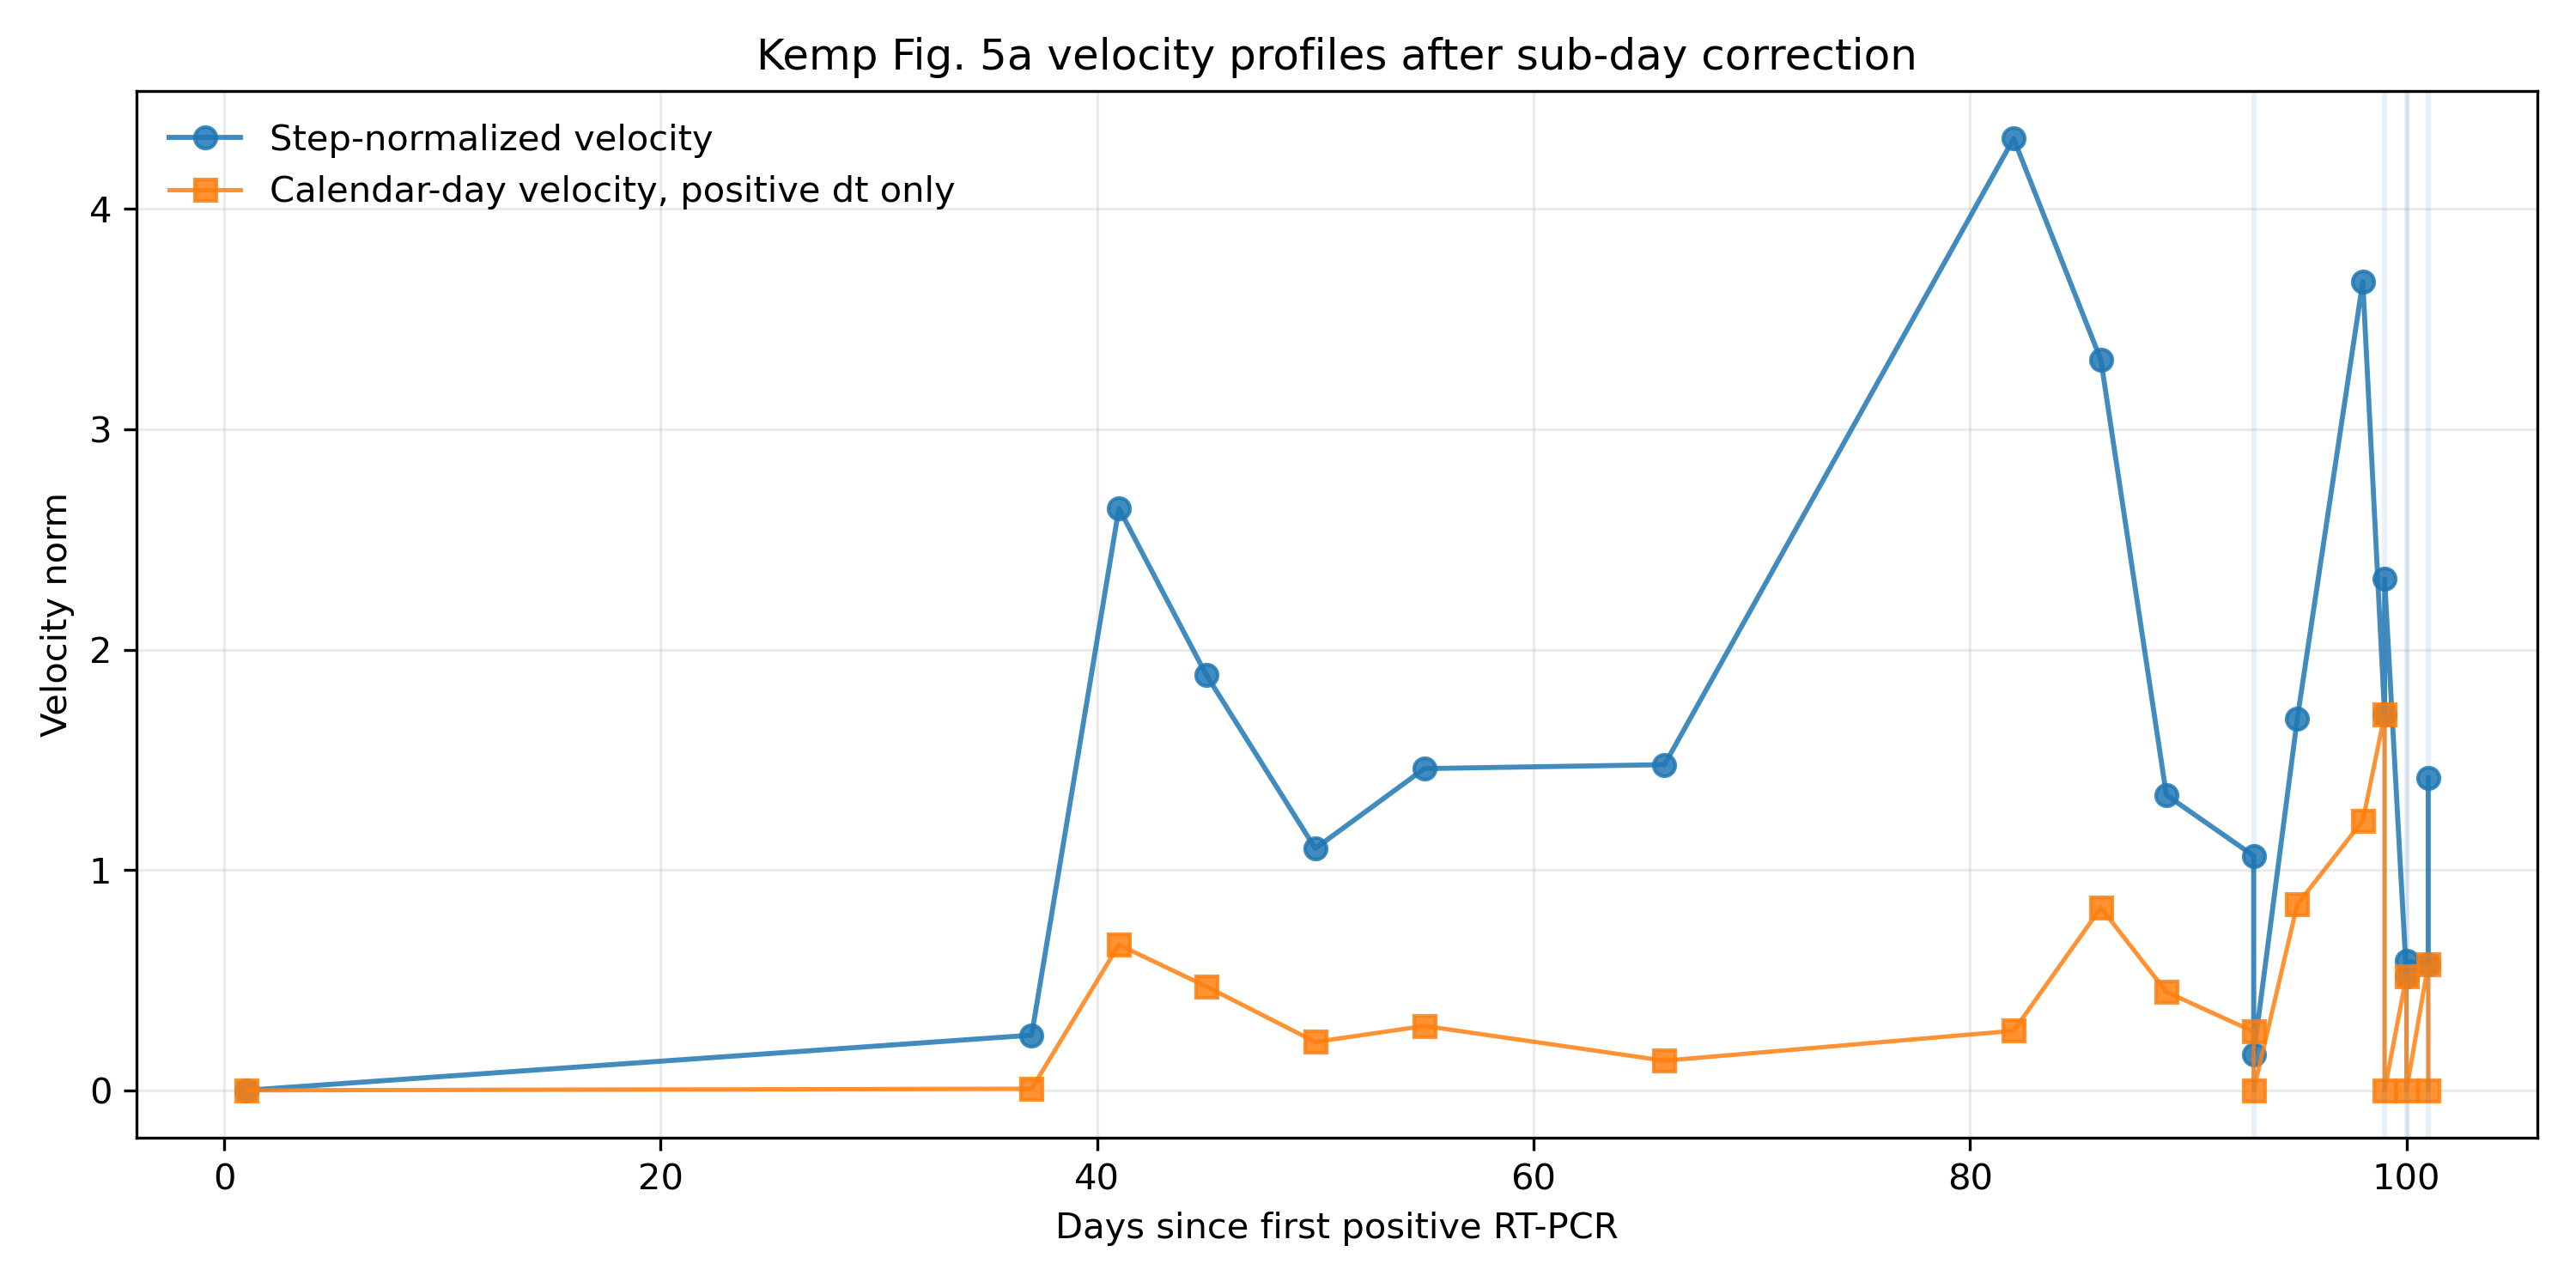
\includegraphics[width=0.9\textwidth]{figures/phase1_sarscov2/kemp_fig5a_velocity_profiles_over_days.png}
\caption{kemp fig5a velocity profiles over days}
\end{figure}

\begin{figure}[h]
\centering
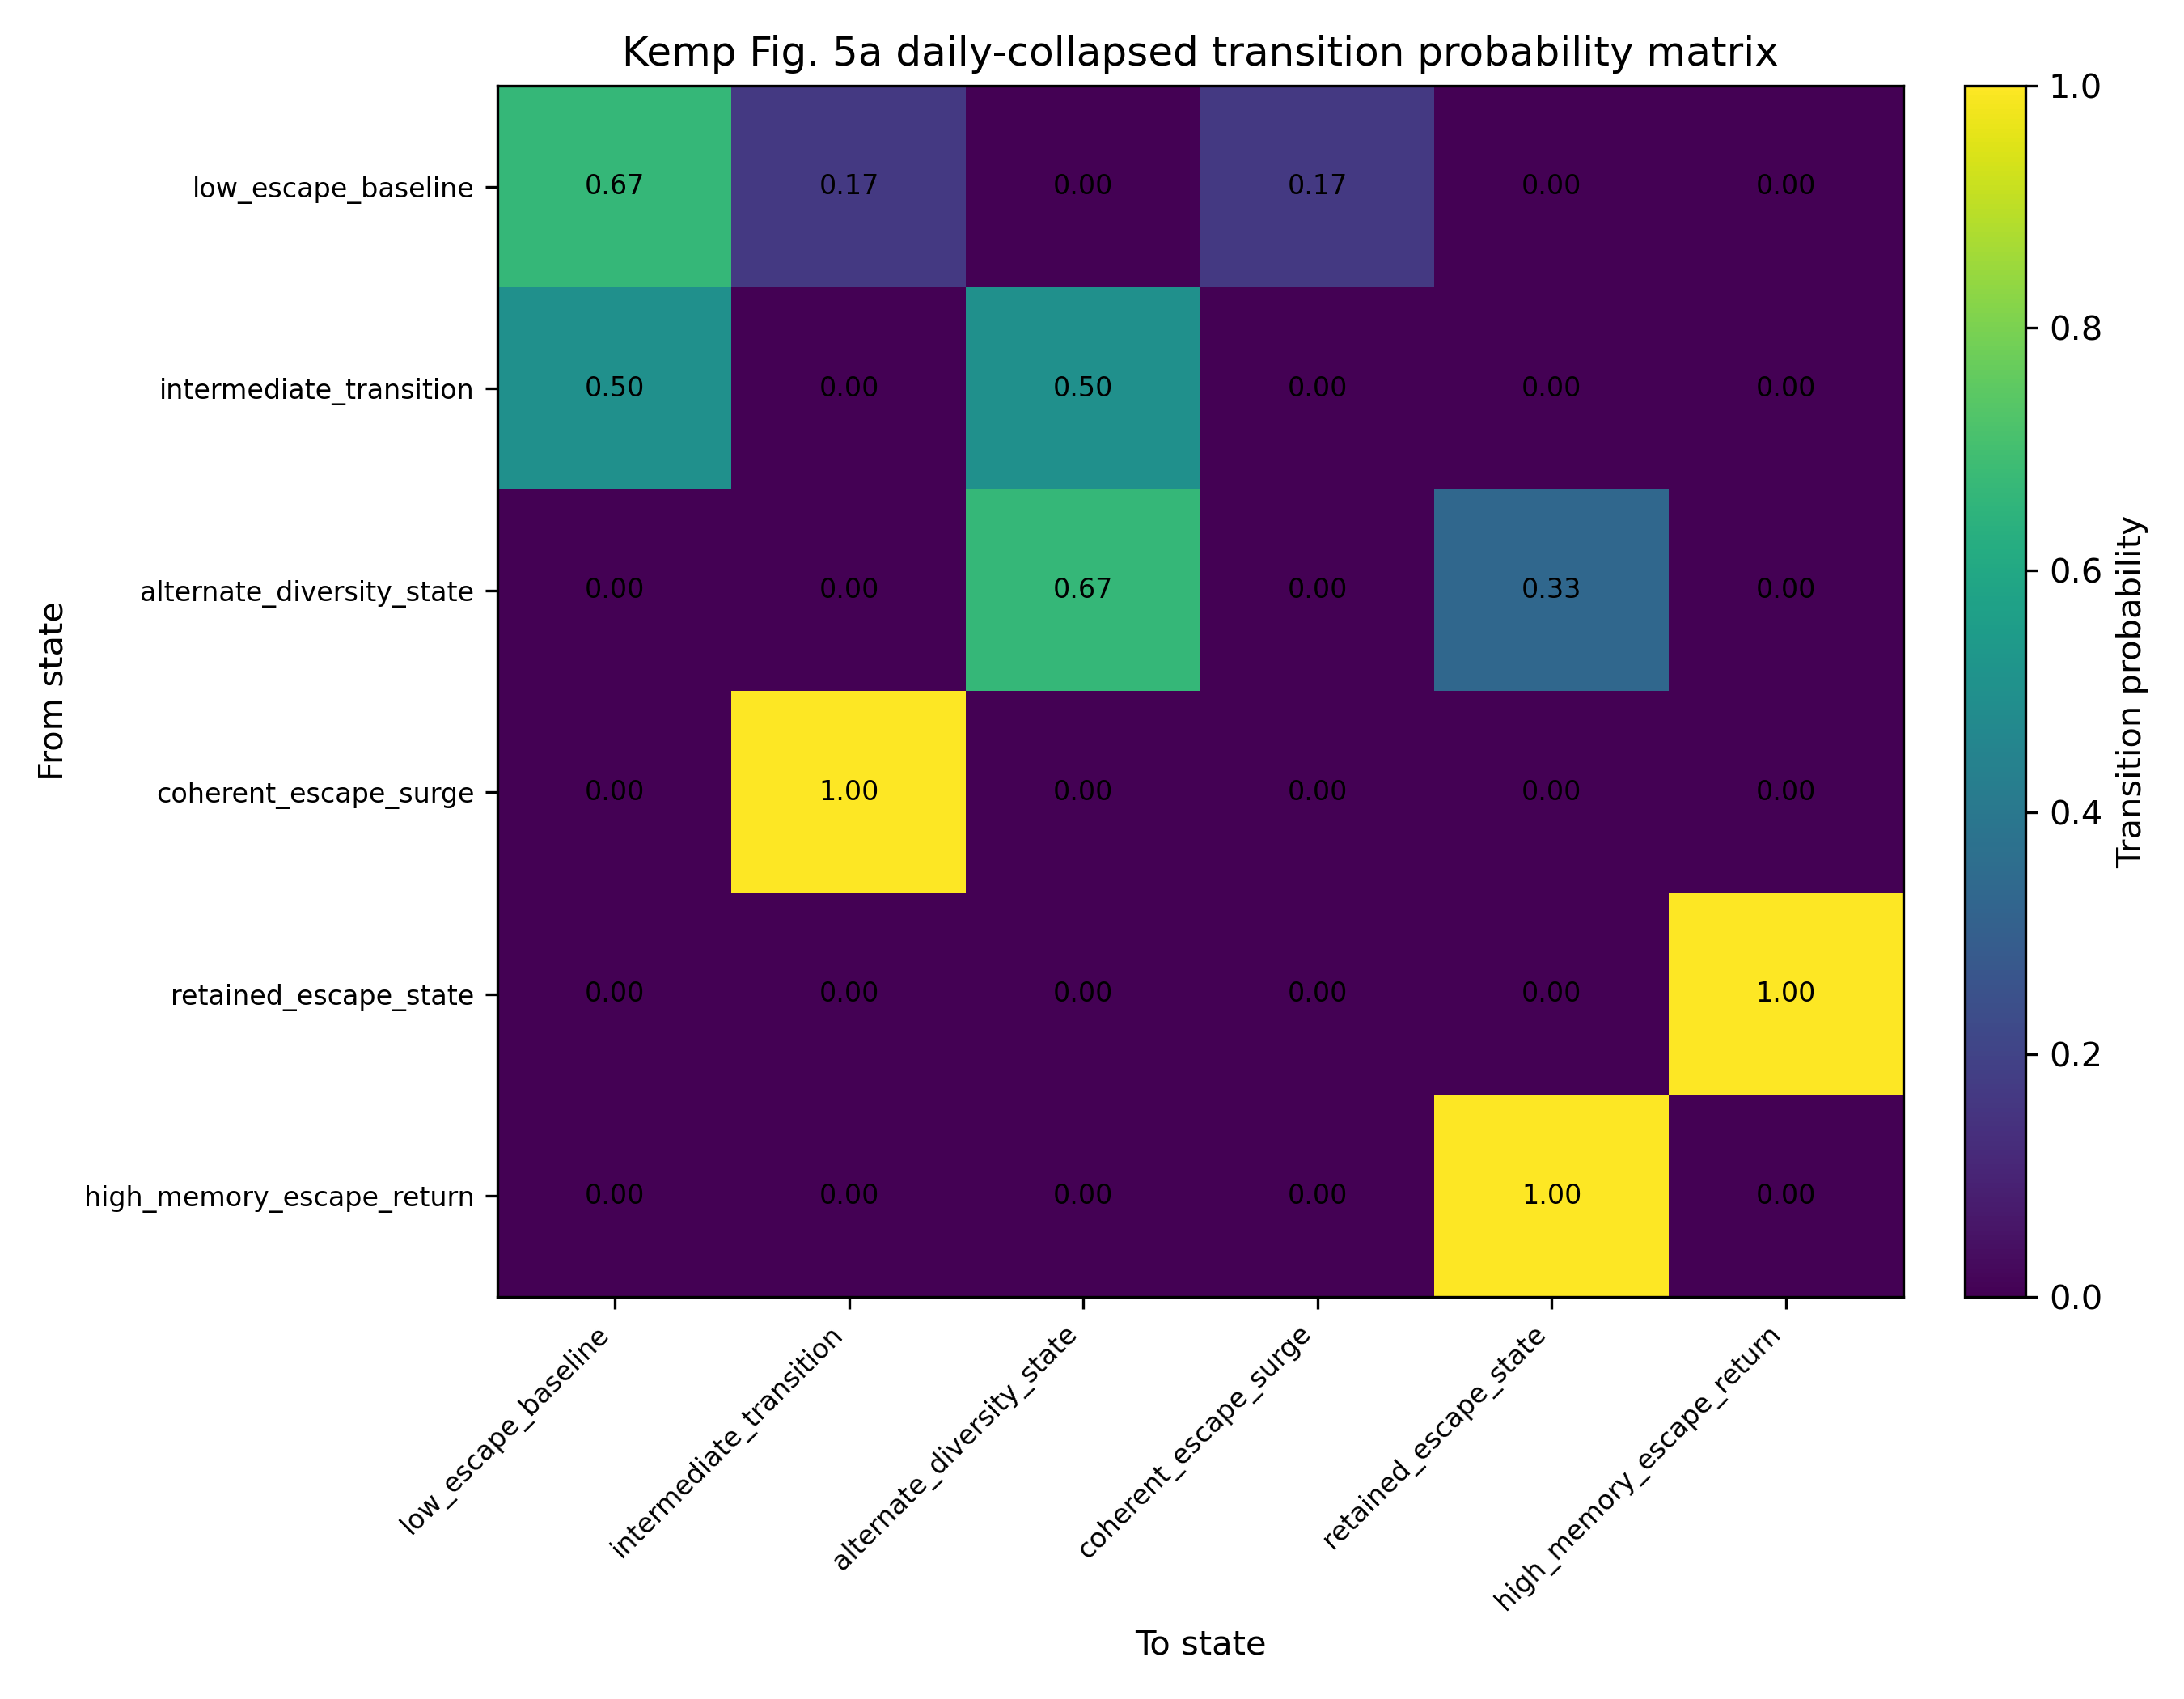
\includegraphics[width=0.9\textwidth]{figures/phase1_sarscov2/kemp_fig5a_daily_collapsed_transition_heatmap.png}
\caption{kemp fig5a daily collapsed transition heatmap}
\end{figure}

\begin{figure}[h]
\centering
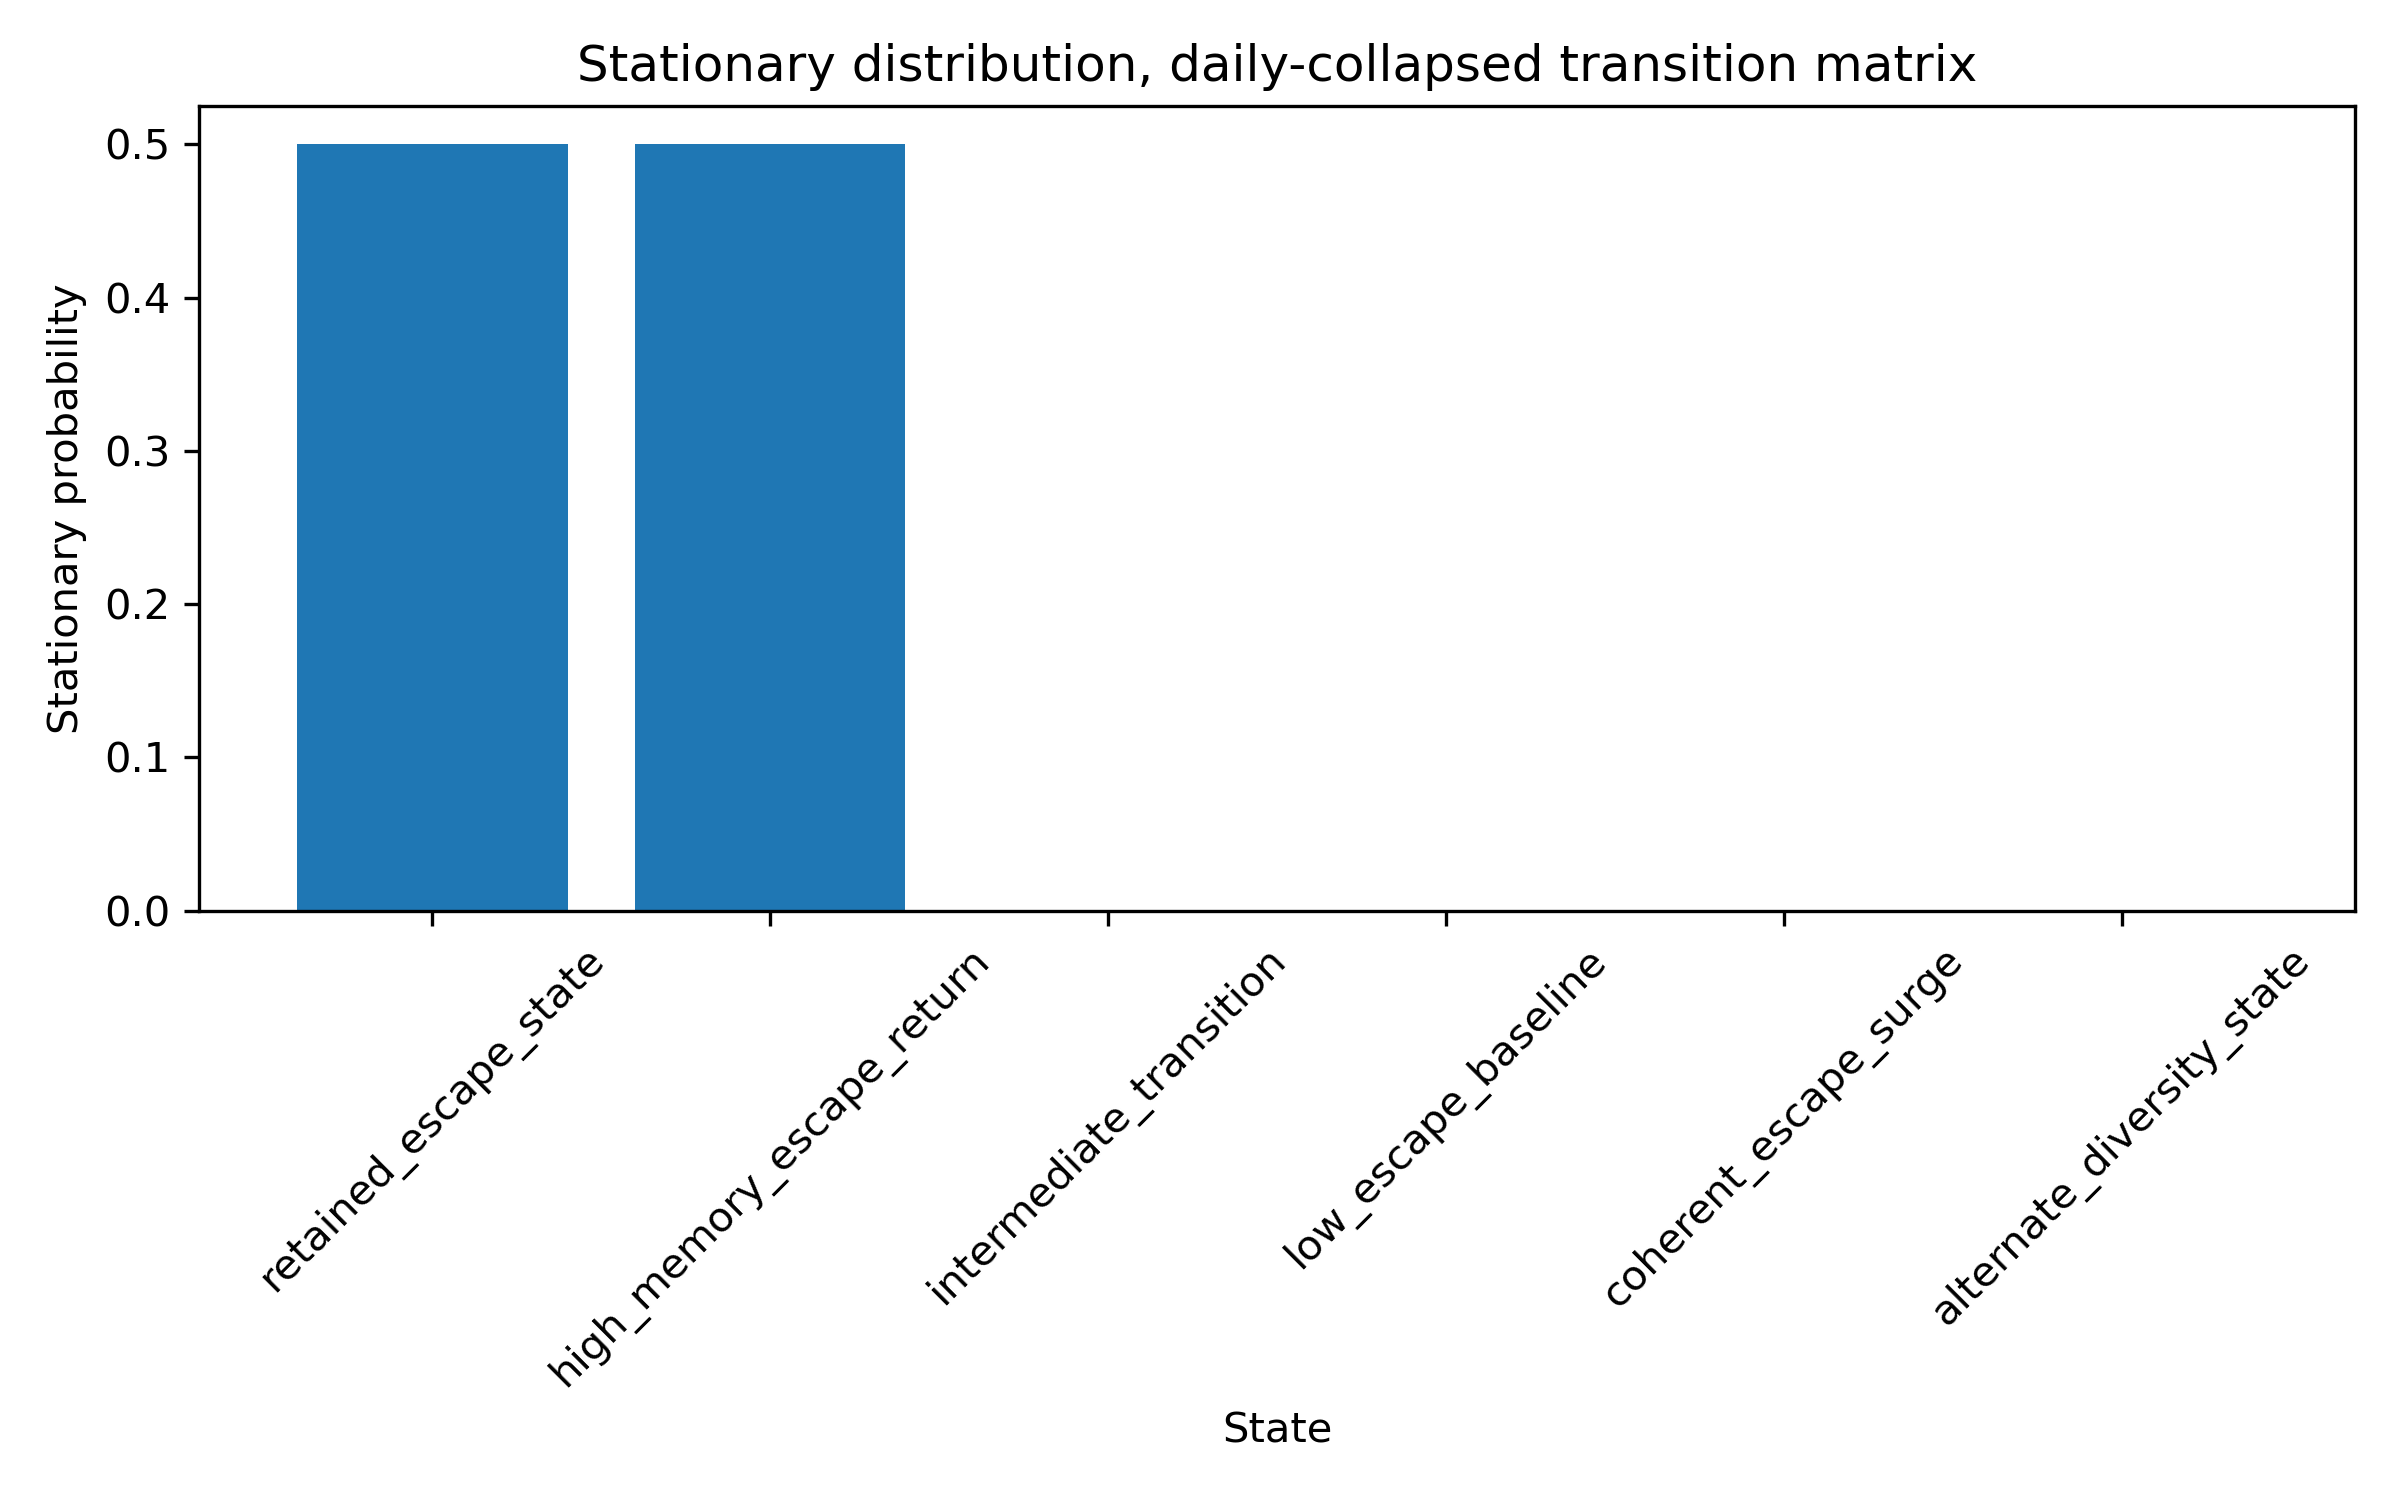
\includegraphics[width=0.9\textwidth]{figures/phase1_sarscov2/kemp_fig5a_daily_collapsed_stationary_distribution.png}
\caption{kemp fig5a daily collapsed stationary distribution}
\end{figure}

\begin{figure}[h]
\centering
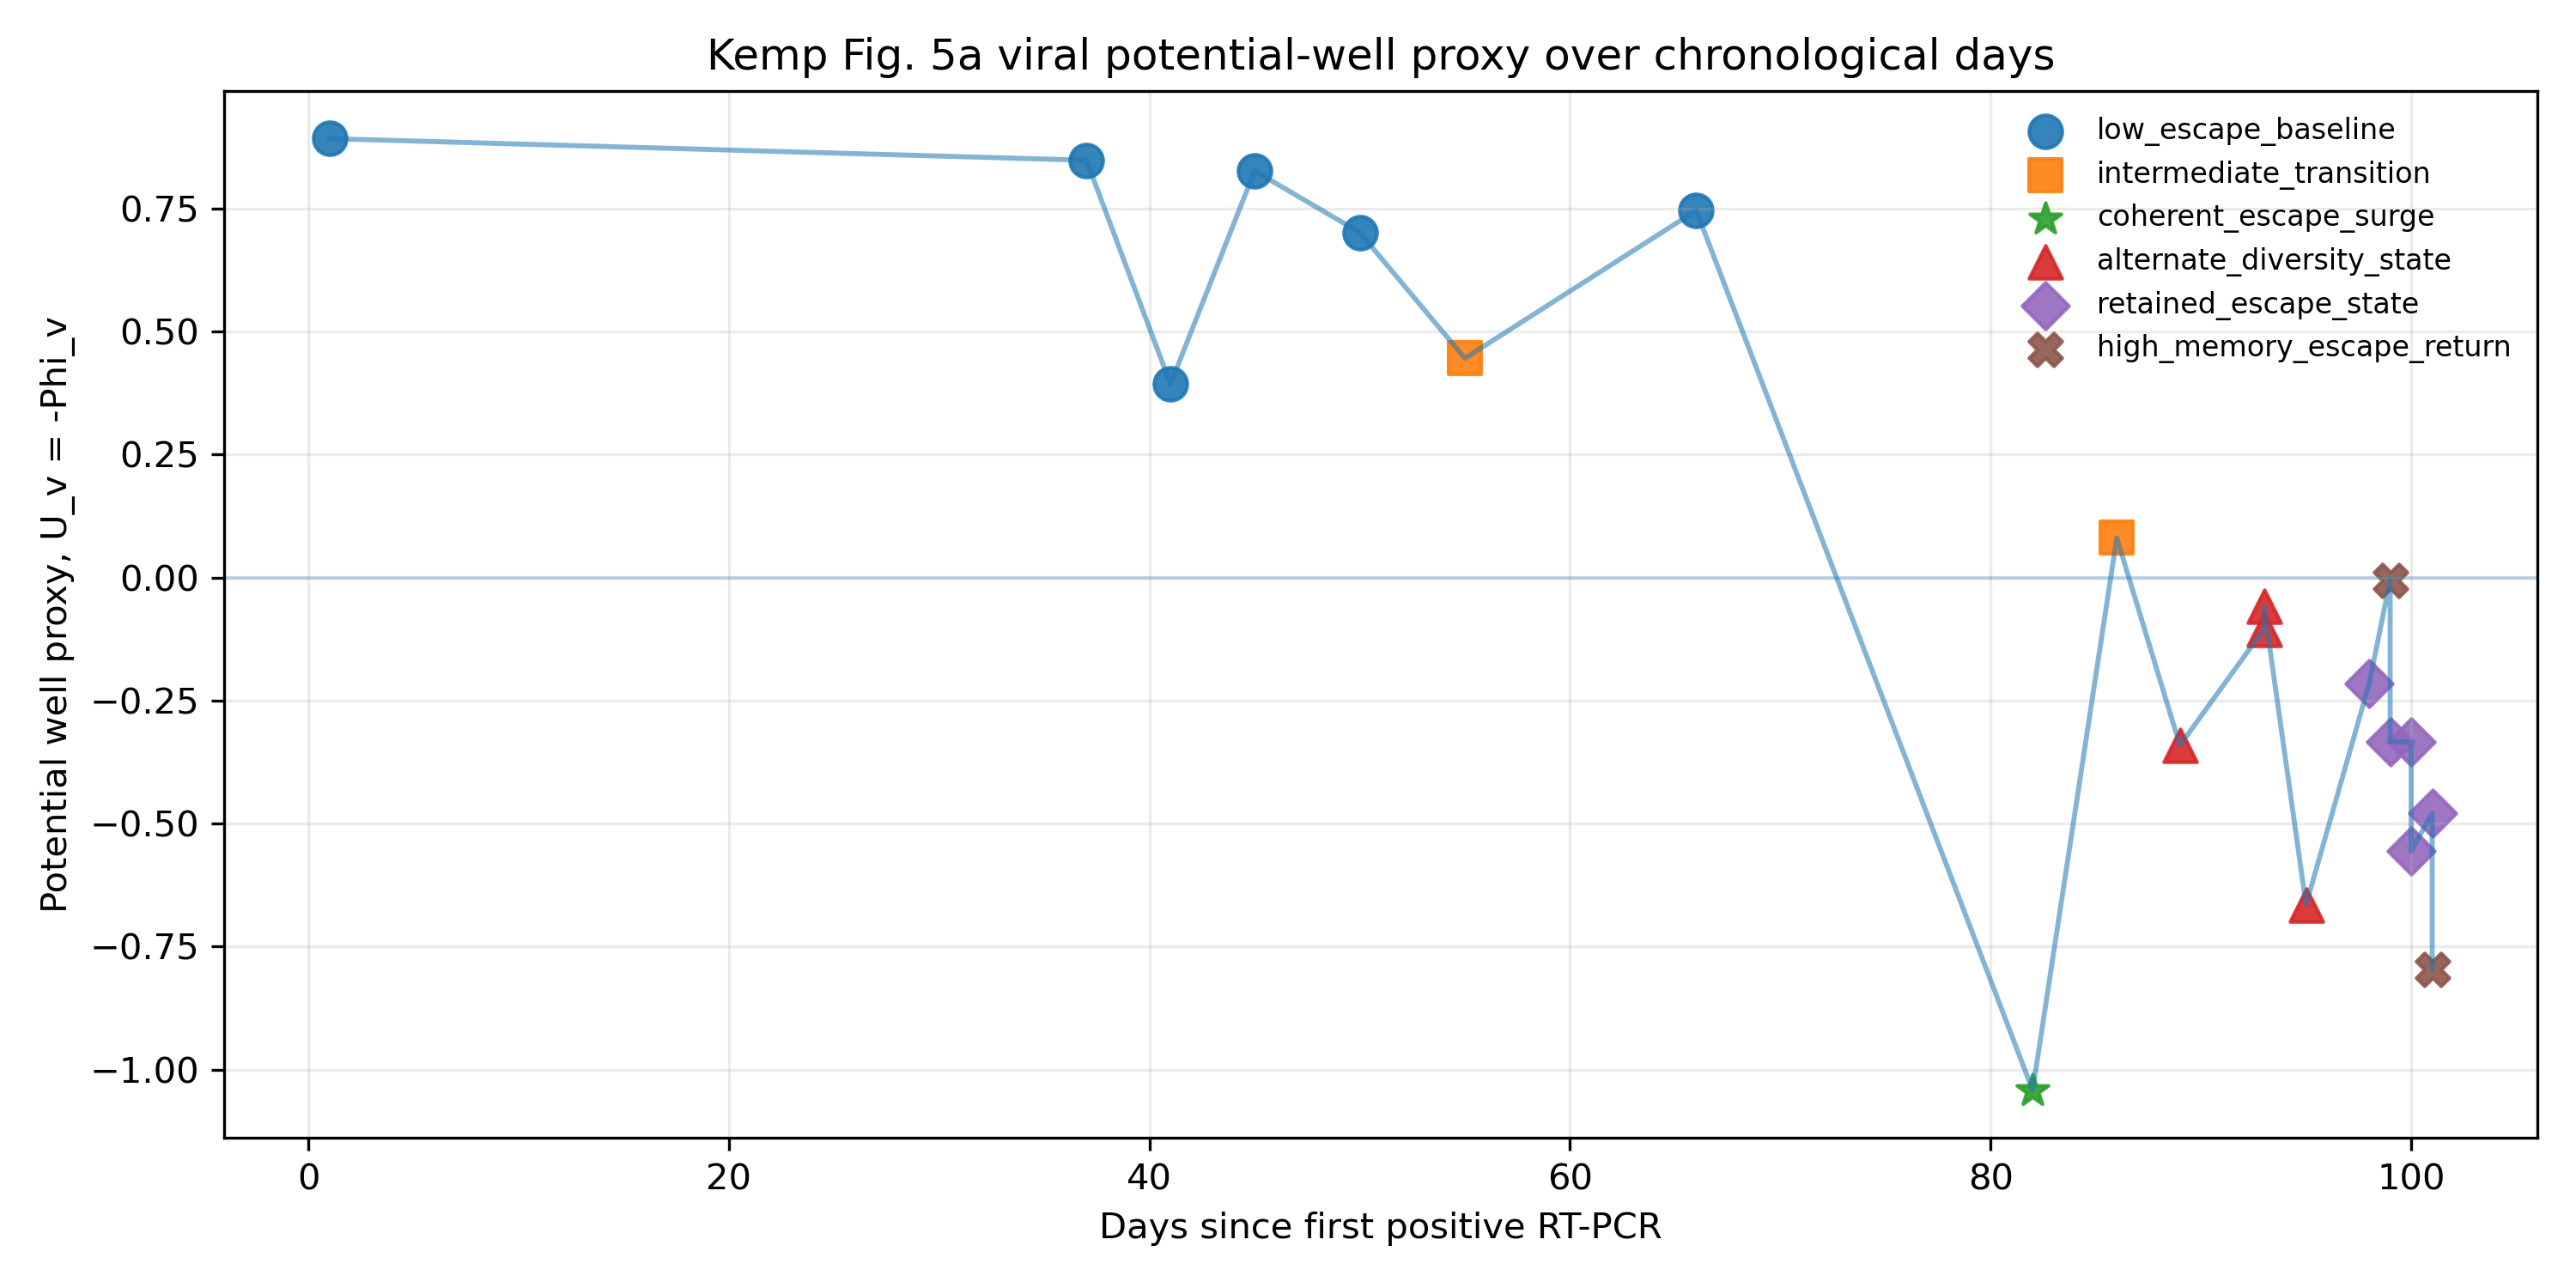
\includegraphics[width=0.9\textwidth]{figures/phase1_sarscov2/kemp_fig5a_potential_well_over_days.png}
\caption{kemp fig5a potential well over days}
\end{figure}

\begin{figure}[h]
\centering
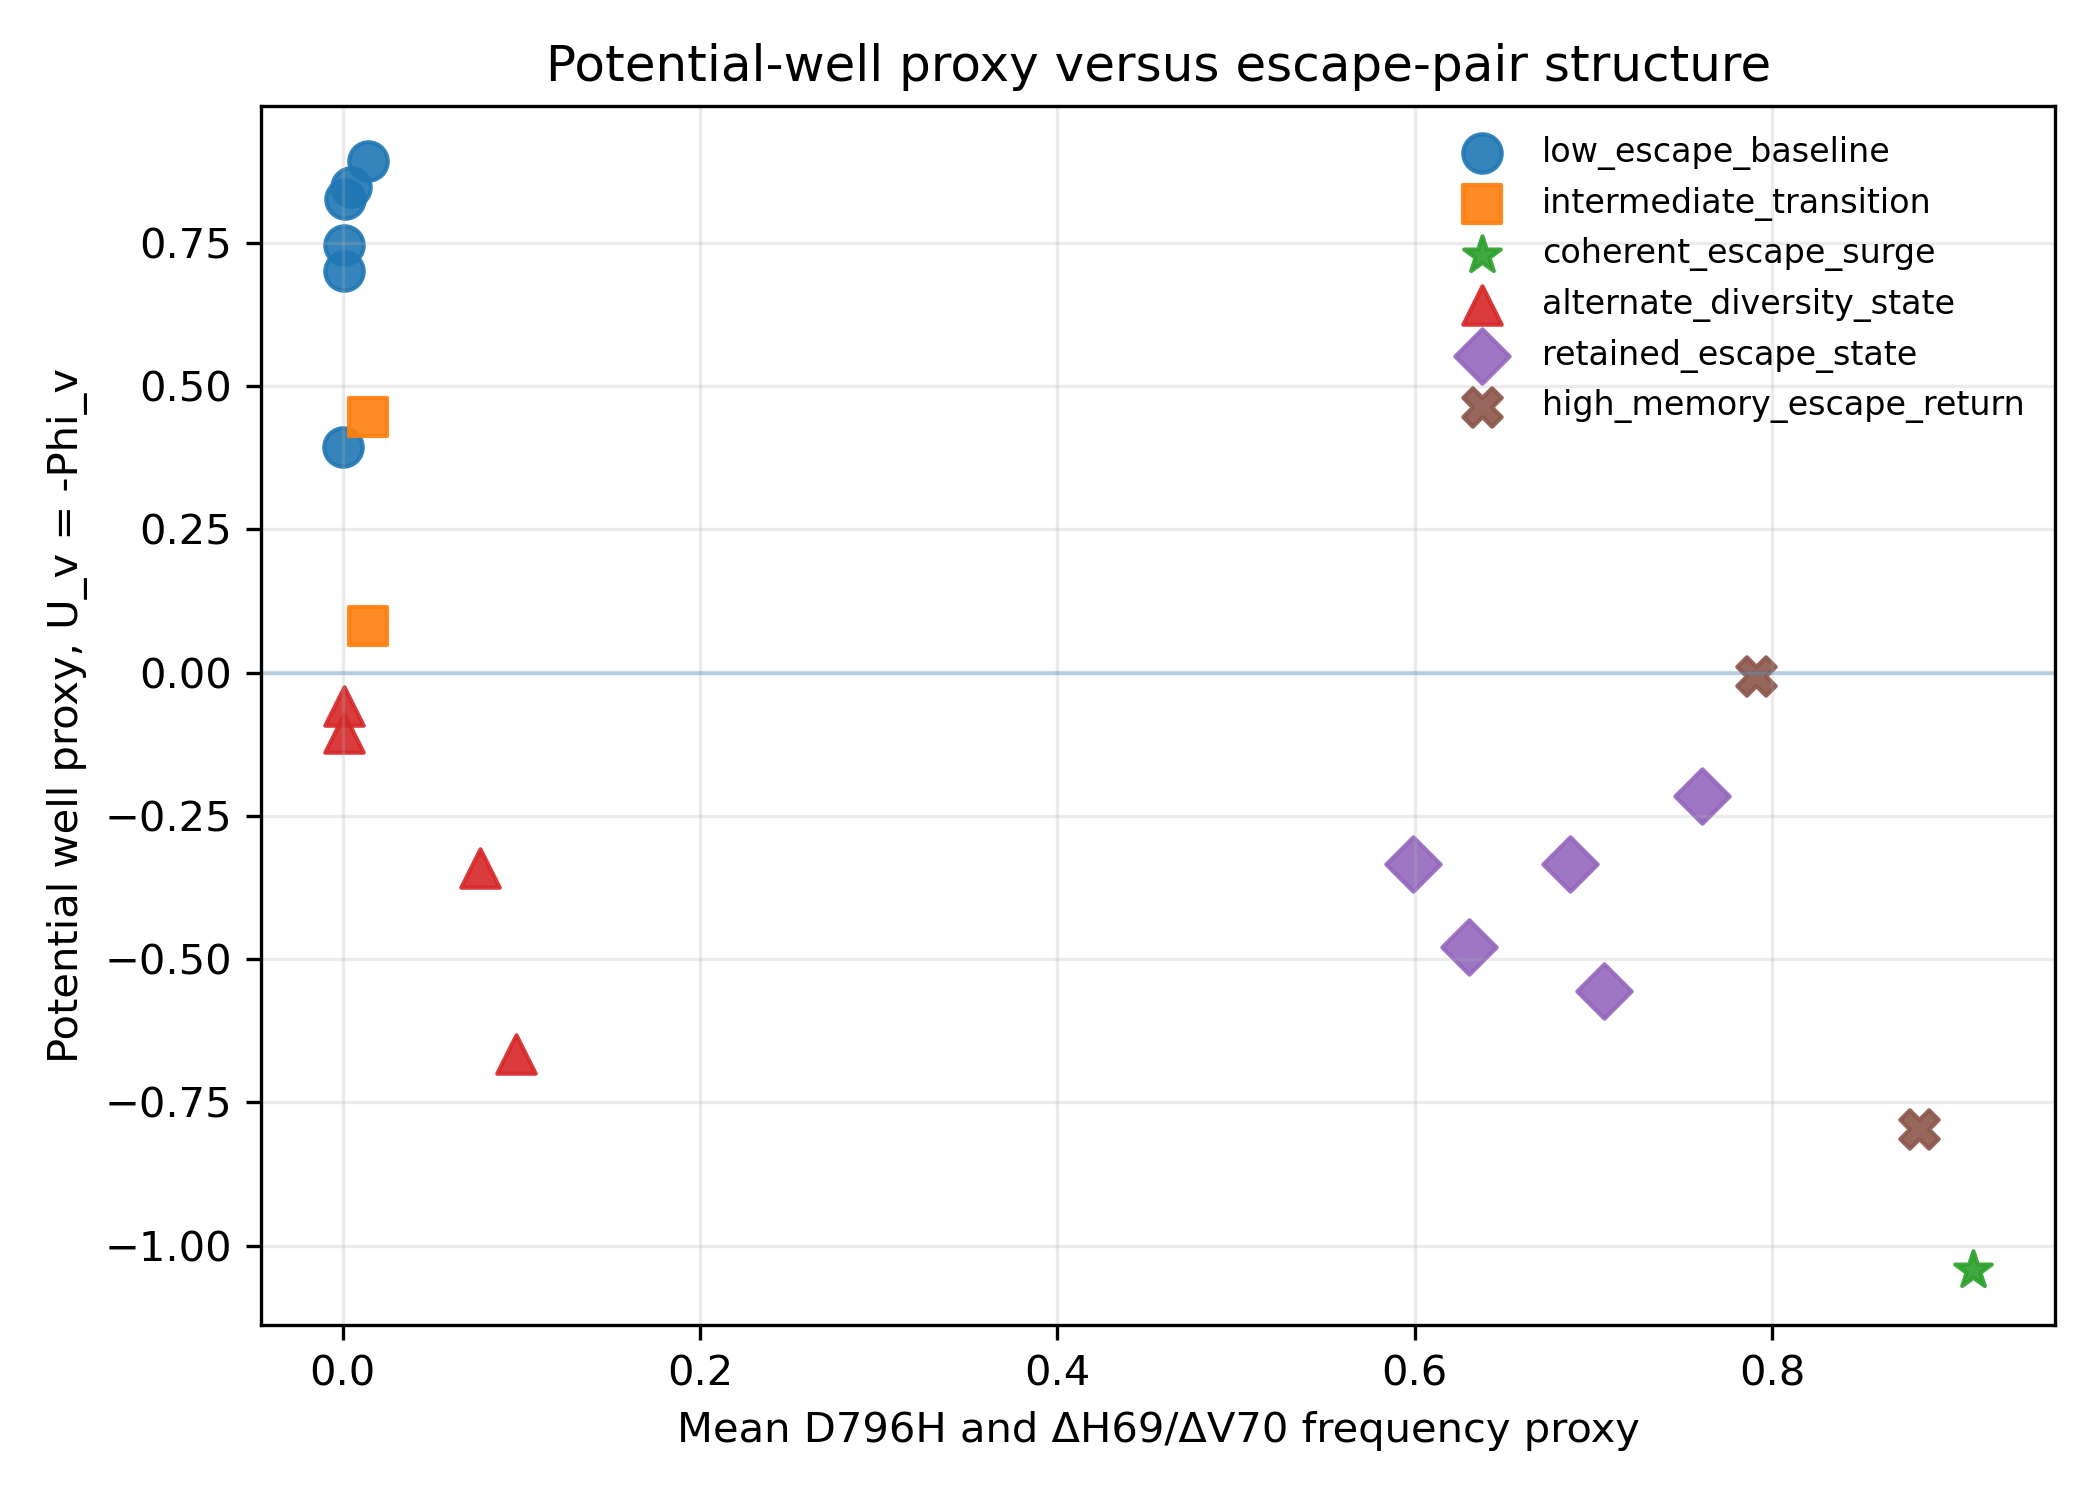
\includegraphics[width=0.9\textwidth]{figures/phase1_sarscov2/kemp_fig5a_potential_vs_escape_pair.png}
\caption{kemp fig5a potential vs escape pair}
\end{figure}

\begin{figure}[h]
\centering
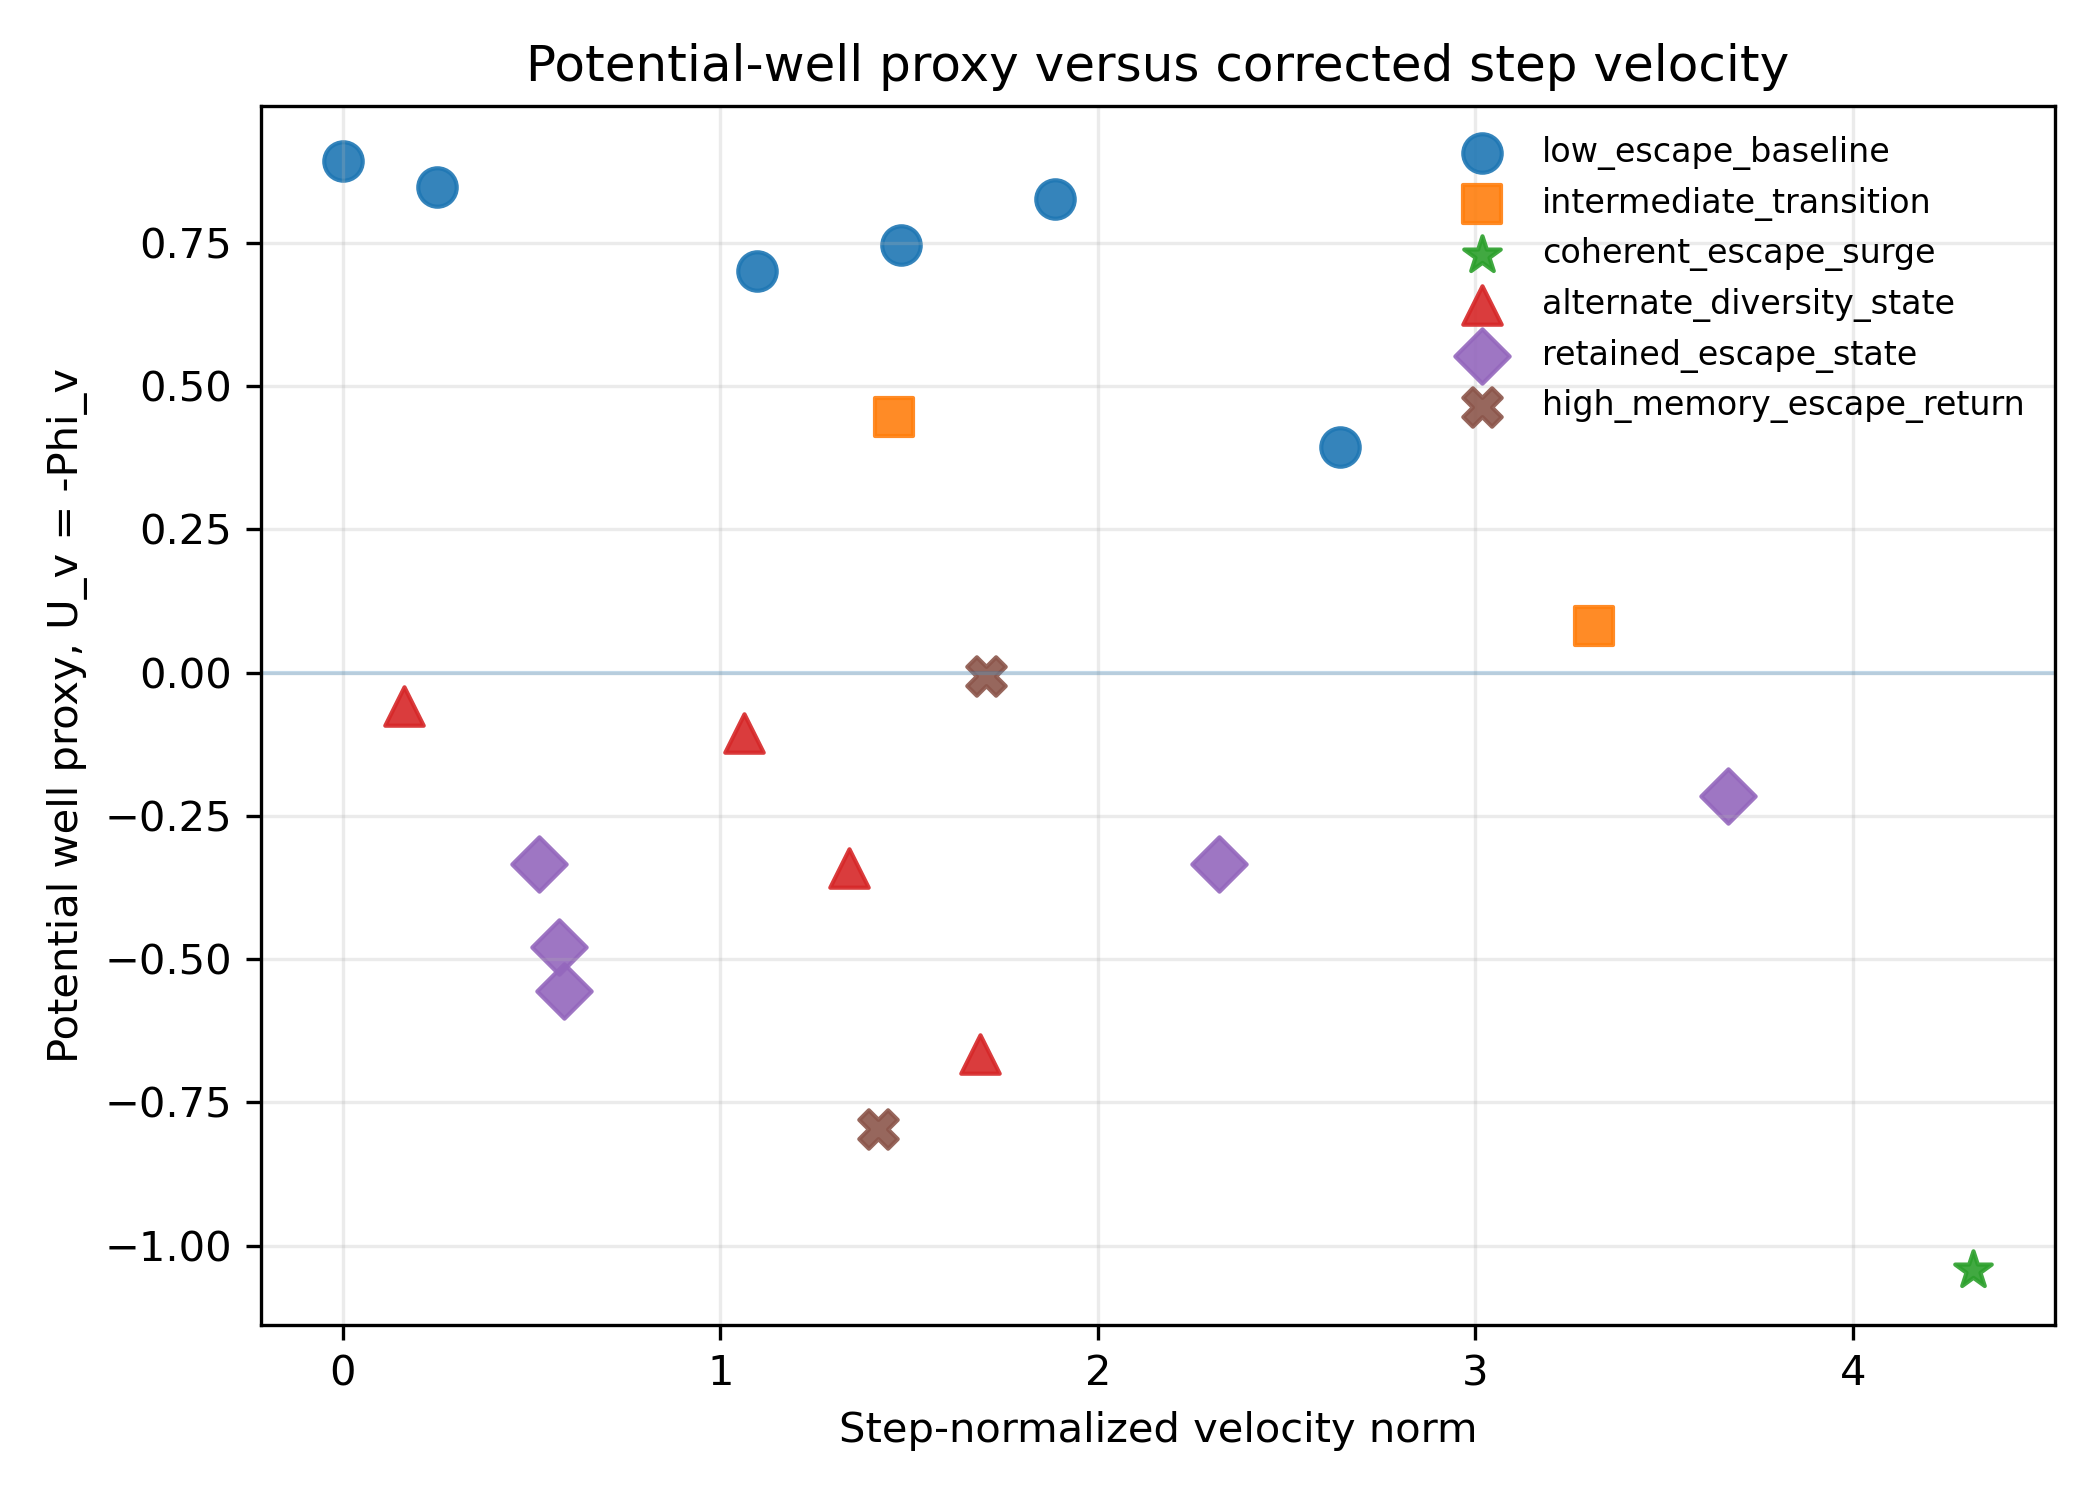
\includegraphics[width=0.9\textwidth]{figures/phase1_sarscov2/kemp_fig5a_potential_vs_step_velocity.png}
\caption{kemp fig5a potential vs step velocity}
\end{figure}

\subsection*{Interpretation boundary}
This Phase I result is a pilot topology from one figure-source reconstruction. It supports continued testing of a viral HRSM memory branch, but it does not prove a universal viral attractor, does not establish clinical phenotype classes, and does not replace raw sequencing analysis.